\documentclass[a4paper, 12pt]{article}
\usepackage[top=1.8cm, bottom=1.8cm, left=1.5cm, right=1.5cm]{geometry}
\usepackage{amsmath}
\usepackage{listings}
\usepackage{float}
\usepackage{tikz}

\begin{document}
	\begin{center}
		Universidade Federal do Rio Grande do Norte
		
		Departamento de Engenharia da Computação e Automação
		
		DCA3703 - Programação Paralela
		
		\textbf{Tarefa 10 - Mecanismos de sincronização: atomic e reduction}
		
		\textbf{Aluno:} Daniel Bruno Trindade da Silva
	\end{center}
	
	\section{Introdução}
	\hspace{0.7cm}O valor de $\pi$ (pi) é uma constante matemática fundamental, frequentemente utilizada em cálculos científicos e de engenharia. Uma forma interessante e didática de estimá-lo é por meio do método de Monte Carlo, que utiliza experimentos estocásticos baseados em geração de números aleatórios para simular eventos e calcular probabilidades. Neste experimento, implementamos três versões paralelas de um estimador de $\pi$ utilizando a API OpenMP, explorando diferentes mecanismos de sincronização para controlar o acesso concorrente às variáveis compartilhadas entre threads.
	
	A primeira versão emprega a diretiva \texttt{\#pragma omp critical}, que garante exclusão mútua, mas pode introduzir gargalos de desempenho. A segunda substitui essa abordagem por \texttt{\#pragma omp atomic}, adequada para operações simples como incrementos. Por fim, a terceira versão utiliza a cláusula \texttt{reduction}, que permite ao compilador otimizar a operação de soma paralela com contadores locais, sendo geralmente mais eficiente. Com isso, buscamos comparar o impacto dessas técnicas tanto em termos de desempenho quanto de produtividade na programação paralela.
	
	\section{Metodologia}
		\hspace{.7cm}O método estocástico de Monte Carlo para estimar o valor de $\pi$ é uma técnica probabilística que usa números aleatórios para resolver um problema matemático. Para estimar $\pi$ utilizaremos um circulo de raio 1 circunscrito em um quadrado de lado 2, ambos posicionados no centro do eixo de coordenadas como mostrado na figura 1: 
	
	
	\begin{center}
		\begin{figure}[H]
			\centering
			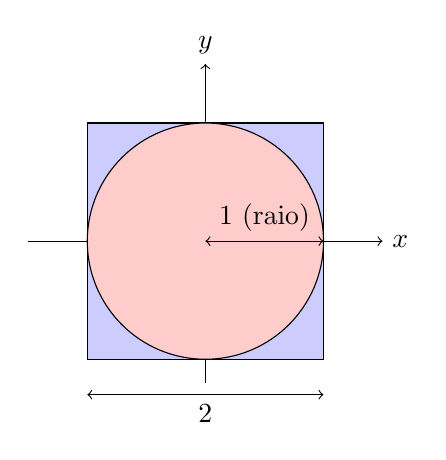
\begin{tikzpicture}[scale=1.5]
				% Eixos coordenados
				\draw[->] (-1.5,0) -- (1.5,0) node[right]{$x$};
				\draw[->] (0,-1.2) -- (0,1.5) node[above]{$y$};
				
				% Quadrado de lado 2 encostado nos eixos
				\draw[fill=blue!20] (-1,-1) rectangle (1,1);
				%\node at (-1,1.2) {Quadrado};
				
				% Círculo de raio 1 à direita do quadrado
				\draw[fill=red!20] (0,0) circle (1);
				%\node at (3,1) {Círculo};
				
				% Marcas de dimensão
				\draw[<->] (-1,-1.3) -- (1,-1.3) node[midway,below]{2};
				%\draw[<->] (0,0) -- (0,1) node[midway,right]{2};
				\draw[<->] (0,0) -- (1,0) node[midway,above]{1 (raio)};
			\end{tikzpicture}
			\caption{Circulo de raio 1 circunscrito em um quadrado de lado 2}
		\end{figure}
	\end{center}
	
	
	Em seguida geraremos muitos pares (x,y) com valores aleatórios entre -1 e 1, ou seja, dentro da área do quadrado, a proporção de pontos encontrados dentro do círculo em relação ao total gerado se aproxima da razão entre as áreas:
	
	\[
	\frac{\text{Pontos no Círculo}}{\text{Total de Pontos}} \approx \frac{\pi}{4}
	\]
	
	\vspace{1.5cm}
	
	Então para estimarmos o valor de $\pi$ pelo método de Monte Carlo temos:
	
	\[
	\pi \approx 4 \times \frac{\text{Pontos no Círculo}}{\text{Total de Pontos}}
	\]
	
	\vspace{.5cm}
	
	Assim, a base de nosso código será composto por um laço de repetição que gerará \textit{n} pares aleatórios (x,y) e testará se os pontos estão dentro ou não do circulo. Ao final utilizaremos a proporção de acertos pelo número de pares (x, y) para estimarmos o valor de $\pi$.
	
	Nesta tarefa, foram desenvolvidas três versões distintas do código, cada uma utilizando um mecanismo diferente de sincronização:
	
	\begin{itemize}
		\item A \textbf{primeira versão} emprega a diretiva \texttt{\#pragma omp critical}, que protege a região crítica onde a variável global é atualizada, garantindo que apenas uma thread por vez execute essa operação.
		
		\item A \textbf{segunda versão} utiliza a diretiva \texttt{\#pragma omp atomic}, que oferece uma forma mais leve de sincronização para operações simples, como a adição à variável global.
		
		\item A \textbf{terceira versão} adota a cláusula \texttt{reduction}, permitindo que cada thread mantenha um contador local, cuja soma final é realizada automaticamente pelo OpenMP, eliminando a necessidade de sincronização explícita.
	\end{itemize}
	
	Sendo assim, a região paralela de nosso código ficou da seguinte forma:
	
	\vspace{.5cm}
	
	\textbf{Versão com \texttt{\#pragma omp critical}}
	
	\begin{verbatim}
		    // Região paralela
		    #pragma omp parallel default(none) shared(hit, seeds)
		    {
		        int tid = omp_get_thread_num();
		        unsigned int seed = seeds[tid];
		        int hit_priv = 0; 
				
		        #pragma omp for
		        for(int i = 0; i < NUM_DOTS; i++){
		            double x = 2.0 * rand_r(&seed) / RAND_MAX - 1.0;
		            double y = 2.0 * rand_r(&seed) / RAND_MAX - 1.0;
					
		            if (x*x + y*y <= 1.0){
		                hit_priv++;
		            }
		        }
				
		        #pragma omp critical
		        {
		            hit += hit_priv;
		        }
		    }
	\end{verbatim}
	
	\vspace{5cm}
	
	\textbf{Versão com \texttt{\#pragma omp atomic}}
	
	\begin{verbatim}
		// Região paralela
		#pragma omp parallel default(none) shared(hit, seeds)
		{
			int tid = omp_get_thread_num();
			unsigned int seed = seeds[tid];
			int hit_priv = 0; 
			
			#pragma omp for
			for(int i = 0; i < NUM_DOTS; i++){
				double x = 2.0 * rand_r(&seed) / RAND_MAX - 1.0;
				double y = 2.0 * rand_r(&seed) / RAND_MAX - 1.0;
				
				if (x*x + y*y <= 1.0){
					hit_priv++;
				}
			}
			
			#pragma omp atomic
				hit += hit_priv;
		}
	\end{verbatim}
	
		\textbf{Versão com \texttt{reduction}}
	
	\begin{verbatim}
		#pragma omp parallel default(none) shared(seeds) reduction(+:hit)
		{
			int tid = omp_get_thread_num();
			unsigned int seed = seeds[tid];
			
			#pragma omp for
			for(int i = 0; i < NUM_DOTS; i++){
				double x = 2.0 * rand_r(&seed) / RAND_MAX - 1.0; // x entre -1 e 1
				double y = 2.0 * rand_r(&seed) / RAND_MAX - 1.0; // y entre -1 e 1
				
				if (x*x + y*y <= 1.0){
					hit++;
				}
			}
		}
	\end{verbatim}

	\section{Resultados}

	Os programas foram executados em um mesmo ambiente computacional, utilizando $1.000.000.000$ (um bilhão) de pontos aleatórios para a estimativa de $\pi$. A Tabela~\ref{tab:tempos} apresenta os tempos de execução observados para cada versão do código, com diferentes mecanismos de sincronização.
	
	\begin{table}[H]
		\centering
		\caption{Tempo de execução para cada versão do código}
		\label{tab:tempos}
		\begin{tabular}{|c|c|}
			\hline
			\textbf{Versão} & \textbf{Tempo de Execução (s)} \\
			\hline
			\texttt{omp atomic}    & 2,0597 \\
			\texttt{omp critical}  & 2,0739 \\
			\texttt{omp reduction} & 2,1183 \\
			\hline
		\end{tabular}
	\end{table}
	
	Embora a expectativa teórica fosse de que a versão com \texttt{reduction} apresentasse o melhor desempenho — devido ao seu alto nível de otimização interna e eliminação de diretivas de sincronização explícitas —, os resultados demonstraram que a versão com \texttt{atomic} foi ligeiramente mais rápida, seguida de perto pela versão com \texttt{critical}, e por último a versão com \texttt{reduction}.
	
	Essas pequenas variações podem ser atribuídas a diversos fatores, como:
	\begin{itemize}
		\item A sobrecarga de criação e gerenciamento dos contadores locais na cláusula \texttt{reduction}, que pode não compensar os ganhos esperados em determinados contextos.
		\item O uso eficiente da operação atômica (\texttt{atomic}) em hardware moderno, que pode apresentar desempenho comparável ou até superior a outras técnicas, especialmente quando a operação protegida é simples.
	\end{itemize}
	
	Apesar das diferenças de tempo serem mínimas (todas próximas de 2 segundos), os resultados mostram que nenhuma técnica é absolutamente superior em todos os contextos, reforçando a importância de avaliar o desempenho prático de cada abordagem dentro do cenário de aplicação específico.

	\section{Conclusão}
	
	A realização deste experimento permitiu explorar, na prática, diferentes estratégias de sincronização em programação paralela com OpenMP. Através da implementação de três versões do estimador de $\pi$ com os mecanismos \texttt{critical}, \texttt{atomic} e \texttt{reduction}, foi possível comparar o impacto de cada abordagem no desempenho da aplicação.
	
	Os resultados demonstraram que, embora a cláusula \texttt{reduction} seja frequentemente considerada a mais eficiente devido à sua capacidade de otimização interna, a versão utilizando \texttt{atomic} apresentou o menor tempo de execução no contexto testado. Isso evidencia que o desempenho real pode variar de acordo com fatores como o tipo de operação sincronizada, a carga de trabalho, o número de threads e as características do hardware utilizado.
	
	Do ponto de vista de produtividade, a cláusula \texttt{reduction} oferece uma sintaxe mais limpa e intuitiva, sendo ideal para operações de agregação simples. Já as diretivas \texttt{critical} e \texttt{atomic} oferecem maior flexibilidade, mas requerem atenção redobrada ao risco de condições de corrida e ao impacto no desempenho.
	
	Em resumo, a escolha do mecanismo de sincronização mais adequado deve considerar tanto a natureza da operação concorrente quanto o equilíbrio entre legibilidade do código e eficiência da execução. Experimentos como este reforçam a importância da análise empírica para embasar decisões de projeto em sistemas paralelos.
	
	
\end{document}